\chapter{Numerical Solutions}
As we are usually interested in finding real (or complex) valued solutions of our systems we also have to look into solving them numerically. This chapter focuses on the numerical solution of the mentioned systems.

We will first focus on methods used to solve a more general problem
\begin{align}
	\label{general numerical problem}
	y'(t) &= f(t,y), \quad t \in [t_0, t_l], \\
	y(t_0) &= y_0.
\end{align}


For this we presume that the function $f(t,y)$ is continuous and Lipschitz, thus \emph{Picard-Lindelöf} gives us, that for every $y_0$ it is uniquely solvable in $[t_0, t_l]$.

Numerical Methods work by discretization, this means we divide the time-intervall into
\begin{displaymath}
	t_0 < t_1 < ... < t_N \leq t_l
\end{displaymath}

and consider approximations $y_m \approx y(t_m)$ for $m=1,...,N$. We call this a \emph{time-grid}. The step-size between two grid-points $t_i - t_j$ might not be choosen equidistant. This can be usefull in certain situations. For simplicity we will non the less assume the stepsize to be equidistant.

\section{Single-Step-Methods}
	The first class of numerical methods we will have a look at are single-step methods. These methods use the previous approximated value $y_j$ and (for implicit methods) also the current approximated value to determine the current value through a \emph{procedural function}.
	
	\begin{definition}
		A numerical method to approximate a differential equation \ref{general numerical problem} on a time-grid $t_0,...,t_l$ with the intermediate values $y_0,...,y_l$ is called a single-step method if it is from the form
		\begin{equation}
			\label{single-step method}
			y_{j+1} = y_j + h_j \phi(t_j,y_j, y_{j+1},h_j).
		\end{equation}
		With the \emph{procedural function} $\phi$. If $\phi$ is not dependent on $y_{j+1}$ then the method is called \emph{explicit}, otherwise it is called \emph{implicit}.
	\end{definition}

	\subsection{Consistency, Stability and Convergence}
	
	To compare different single-step methods we have to define some notions to compare their quality. This leads to the definition of the error of the mehtod, its consistency and its convergence.
	
	\begin{definition}\label{Discretization_Error_SingleStep}
		Let $\tilde{y}_{m+1}$ be the result of one step of \ref{single-step method} with the exact start-vector $y_m = y(t_m)$ then
		\begin{equation}
			\label{local discretization error single step}
			le_{m+1} = le(t_m+h) = y(t_{m+1}) - \tilde{y}_{m+1}, \quad m = 0,...,N-1
		\end{equation}
		is called the \emph{local discretization error} of the single step method at the point $t_{m+1}$.
	\end{definition}

	The error encodes how far off the numerical method is from the true value of the solution. In real applications this solution is usually not known. This shows how important error bounds for numerical methods can be.

	\begin{definition}\label{Consistency_SingleStep}
		A single-step method is called \emph{consistent} if for all initial value problems \ref{general numerical problem} 
		\begin{equation}
			\lim\limits_{h \to 0} \frac{||le(t+h)||}{h} = 0 \quad \text{for} \quad t_0 \leq t \leq t_l
		\end{equation}
		holds.\newline
		It is called \emph{consistent of order p}, if for a sufficiently smooth function $f$
		\begin{equation}
			||le(t+h)|| \leq Ch^{p+1} \quad \text{for all} \quad h \in \mathopen{(} 0,H \mathclose{]} \quad \text{and} \quad t_0 \leq t \leq t_l - h
		\end{equation}
		holds with $C$ not dependent on $h$.
	\end{definition}

	Consistency aims to give insight in how similar the problem that the numerical methods solves it to the real problem that we want the solution from. 

	\begin{definition}\label{Convergence_SingleStep}
		A single-step method is called \emph{convergent}, if for all initial value problems \ref{general numerical problem} for the \emph{global discretization error}
		\begin{displaymath}
			e_m = y(t_m)-y_h(t_m)
		\end{displaymath}
		holds that
		\begin{displaymath}
			\max\limits_{m}||e_m|| \to 0 \quad \text{for} \quad h_{max} \to 0.
		\end{displaymath}
		The single-step method is called to have the \emph{convergence order} $p$, if
		\begin{displaymath}
			\max\limits_{m} ||e_m|| \leq C h_max^p \quad \text{for} \quad h_{max} \in \mathopen{(} 0,H \mathclose{]} \quad \text{with} \quad t_0 \leq t_m \leq t_l
		\end{displaymath}
		with the constant $C$ not dependent on the step size $h$.
	\end{definition}

	As the name suggestes convergence tries to quantify how far off a numerical solution is from the real solution of a system. A very interesting result follows if we also require the Single-Step Method to be stable.
	
	\begin{definition}\label{Discrete_Stability_SingleStep - lecture notes for numpdgl}
		A Single-Step Method is called \emph{(discretely) stable} if for grid-functions $y_h$ and $\tilde{y}_h$ with
		\begin{align}
			y_{i+1} &= y_i + h \phi(t_i, y_i), \\
			\tilde{y}_{i+1} &=  \tilde{y}_i + h [\phi(t_i, \tilde{y}_i) + \theta_i],
		\end{align}
		and perturbations $\theta_i = \theta_h(t_i)$ of the right side as well as a bounded perturbation in the staring-values $y_0 - \tilde{y}_0$ the Error is bounded by
		\begin{displaymath}
			||y_h - \tilde{y}_h||_{\infty,h} \leq C (||y_0 - \tilde{y}_0||_{l^2} + ||\theta_h||_{\infty,h}
		\end{displaymath}
		with a constant $C$ which is not dependent on $h$.
	\end{definition}
	
	For Single-Step Methods which are consistent and stable we obtain the following convergence theorem.
	
	\begin{theorem}[Lax-Richtmyer]\label{Lax-Richtmyer}
		A consistent (with order $p$) and discretely stable Single-Step Method is convergent (with order $p$). (assuming smootheness of the solution $y$)
	\end{theorem}
	
	This theorem is due to Lax and Richtmyer. The converse of this statement is also true. 

	\subsection{further stability properties}
		from numpdgl skript \\
		In this section we consider the following simple problem
		\begin{align}
			u' &= \lambda u, \quad t > 0 \\
			u(0) &= u_0
		\end{align}
		with $\lambda \in \mathbb{C}$ and $u_0$ fixed.
		
		\begin{definition}
			\begin{enumerate}
				\item 
				If a single-step method can be written in the form
				\begin{equation}
					u_{i+1} = R(z) u_i, \quad z:= h*y
				\end{equation}
				then we call $R: \mathbb{C} \to \mathbb{C}$ the \emph{stability function} of the single-step method.
				\item 
				The set
				\begin{equation}
					S := {z \in \mathbb{C} : |R(z)| \leq 1}
				\end{equation}
				is called the region of stability of the method.
				\item 
				A single-step method is called
				\begin{itemize}
					\item \emph{0-stable}, if $0 \in S$.
					\item \emph{A-stable}, if $\mathbb{C}^- \subset S$.
					\item \emph{L-stable}, if $R(z) \to 0$ for $Re(z) \to -\infty$.
				\end{itemize}
			\end{enumerate}
		\end{definition}

	\subsection{Runge-Kutta Methods}
		A very prevalent family of numerical single-step methods are the \emph{Runge-Kutta} methods. 
		
		%\begin{figure}
		%	\centering
		%	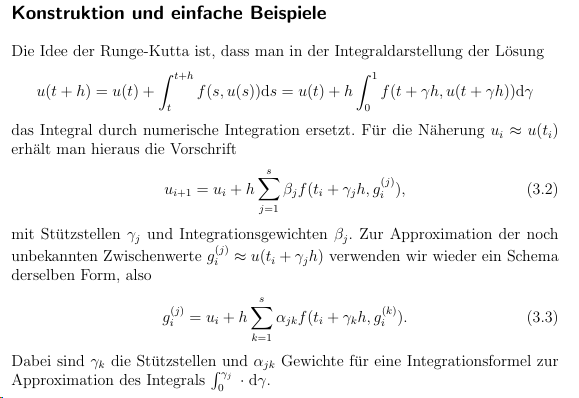
\includegraphics[width=0.7\linewidth]{screenshot026}
		%	\caption{}
		%	\label{fig:screenshot026}
		%\end{figure}
		
		\begin{definition}
			Let $s \in \mathbb{N}$. A single-step method of the form
			\begin{align}
				y_{m+1} = y_m + h \sum_{i=1}^{s} b_i f(t_m + c_ih, y_{m+1}^{(i)}) \\ 
				y_{m+1}^{(i)} = y_m +  \sum_{j=1}^{s} a_{ij} f(t_m + c_jh, y_{m+1}^{(j)})
			\end{align}
			is called a \emph{Runge-Kutta Method} with $s$ steps.
		\end{definition}
		
		We usually collect the coefficients into the vectors and matrices $c=(c_1, ...,c_s)$, $A = (a_{ij})_{ij}$ and $b=(b_1, ..., b_s)$.
		
		If $A$ is a strictly lower triangle matrix, this means for all $j \geq i$ holds $a_{ij} = 0$ then the Runge-Kutta method is explicit, otherwise it is implicit. In general implicit Runge-Kutta methods might need more computational effort because to calculate $y_m^{(i)}$ a nonlinear system of equations has to be solved. But in contrast those methods can also lead to very good stability characteristics.
		
		\begin{lemma}\cite{NumerikGewöhnlicherDifferentialgleichungen}
			A Runge-Kutta mehtod is consistent, if and only if
			\begin{displaymath}
				\sum_{i=1}^{s} b_i = 1
			\end{displaymath}
		\end{lemma}
	
		The coefficients of a Runge-Kutta method are usually represented in the \emph{Butchertableau}, which was introduced by John C. Butcher and has the following form.
		
		\begin{displaymath}
			\begin{array}{c|ccc}
				c_1 & a_{11} & \dots & a_{1s} \\
				\vdots & \vdots & & \vdots \\
				c_s & a_{s1} & \dots & a_{ss} \\
				\hline
				 & b_1 & \dots & b_s
			\end{array}
			\qquad
			\text{of in matrix form}
			\qquad
			\begin{array}{c|c}
				c & A \\
				\hline
				 & b
			\end{array}
		\end{displaymath}
	
		Their stability can directly be derived from the butcher tableau. The stability function of an arbitrary m-stage Runge-Kutta method has the form
		\begin{displaymath}
			R(z) = 1+zb^\top (I_m-zA)^{-1}e
		\end{displaymath}
	
		where $e = (1,...,1)$.
		
		\textbf{Remark:} The trapezoidal rule is a widely used Runge-Kutta method which we can also consider as a multistep-method. It will be discussed later on.
	
			
\section{Multistep-Methods}
	based on chapter 4 of book num gew dgl steif nichtsteif \newline
	Linear multistep methods use approxiamtions $u_{m+l}$ along the gridpoints $t_{m+l}, \quad l=0,1,...,k-1$ to calculate the new approximation $u_{m+k}$ at $t_{m+k}$. We will first discuss topics related to the order of the methods depending on its parameters, stability and convergence.
	
	\begin{definition}
		For given $\alpha_0, ..., \alpha_k$ and $\beta_0, ..., \beta_k$ the iteration rule
		\begin{equation}
			\label{linear-multistep-method}
			\sum_{l=0}^{k} \alpha_l u_{m+l} = h \sum_{l=0}^{k} \beta_l f(t_{m+l}, u_{m+l}), \quad m=0,1,...,N-k
		\end{equation}
		is called a \emph{linear multistep method} (linear k-step method). It is always assumed that $\alpha_k \neq 0$ and $|\alpha_0| + |\beta_k| > 0$. If $\beta_k=0$ holds, then the method is called explicit, otherwise implicit.
	\end{definition}
	
	A linear multi-step method consists of two parts:
	\begin{enumerate}
		\item In the \emph{starting-phase} approximations $u_1,...,u_{k-1}$ for the first $k-1$ gridpoints $t_l = t_0+th, l=1,...,k-1$ are calculated using a single-step method. For example using an explicit Runge-Kutta Method or a multi-step method with fewer steps.
		
		\item  In the \emph{run-phase} the multi-step formula is used to determine new approximations $u_{m+k}$ for the gridpoint $t_{m+k}$
	\end{enumerate}
	
	For theoretical analysis of the multi-step methods we consider the generating polynomials
	\begin{equation}
		\rho(x) := \sum_{l=0}^{k} \alpha_l x^l
	\end{equation}
	\begin{equation}
		\sigma(x) := \sum_{l=0}^{k} \beta_l x^l
	\end{equation}
	
		
	
	\subsection{Consistency, Stability and Convergence}
	\cite{NumerikGewöhnlicherDifferentialgleichungen}
	
	Again we need to define the properties consistency, stability and convergence for this method.
	\begin{definition}
		Let $\tilde{y}_{m+k}$ be the result of one step of the multi-step method \ref{linear-multistep-method} with the start-vectors $y_m = y(t_m)$. This means
		\begin{displaymath}
			\alpha_k \tilde{u}_{m+k} = \sum_{l=0}^{k-1} \left( h \beta_l f(t_{m+l}, y(t_{m+l})) - \alpha_l y(t_{m+l}) \right) + h \beta_k f(t_{m+k}, \tilde{u}_{m+k}) .
		\end{displaymath}
		Then
		\begin{displaymath}
			le_{m+k} = le(t_{m+k}) = y(t_{m+k}) - \tilde{u}_{m+k}, \quad m=0,1,...,N-k
		\end{displaymath}
		is called the \emph{local discretization error} (local error) of the linear multi-step method \ref{linear-multistep-method} at the point $t_{m+k}$.
	\end{definition}
	
	We will assign the linear difference operator
	\begin{equation}
		L[y(t),h] = \sum_{l=0}^{k} \left( \alpha_l y(t+lh) - h \beta_l y'(t+lh) \right)
	\end{equation}
	to the local discretization error. Using this we gain the following definition.

	\begin{definition}
		A linear multi-step method is called \emph{preconsistent} if for all functions $y(t) \in C^1[t_0,t_l]$
		\begin{displaymath}
			\lim\limits_{h \to 0} L[y(t),h]=0
		\end{displaymath}
		holds. It is called \emph{consistent}, if for all functions $y(t) \in C^2[t_0,t_l]$
		\begin{displaymath}
			\lim\limits_{h \to 0} \frac{1}{h} L[y(t),h] = 0
		\end{displaymath}
		holds. It has the \emph{consistency order p}, if for all functions $y(t) \in C^{p+1}[t_0, t_l]$
		\begin{displaymath}
			L[y(t),h] = \mathcal{O}(h^{p+1}) \quad \text{for} \quad h \to 0
		\end{displaymath}
		holds.
	\end{definition}

	From the generating polynomials we can derive simple consistency conditions
	\begin{displaymath}
		\rho(1) = 0 \quad \text{and} \quad \rho'(1) = \sigma(1).
	\end{displaymath}

	Of course we also need convergence of such methods.
	
	\begin{definition} \label{def: LMSV convergence}
		We say that a linear multi-step method is convergent if for a solution $y$ of the problem a solution vector created by an LMSV $y_j$ for $j \in {0,...,k}$ we have that
		\begin{displaymath}
			\lim\limits_{h \to \infty} \max_{0 \leq j \leq k} ||y(t_j) - y_j|| = 0.
		\end{displaymath}
	\end{definition}
	
	%\begin{figure}
	%	\centering
	%	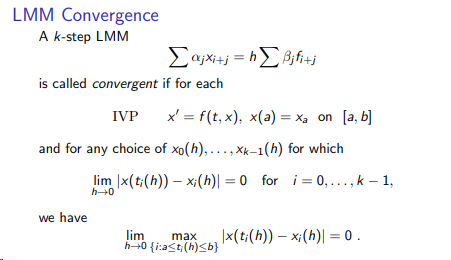
\includegraphics[width=0.7\linewidth]{screenshot025}
	%	\caption{}
	%	\label{fig:screenshot025}
	%\end{figure}
	
	The discrete stability is also very similar to the single-step methods.
	\begin{definition} \label{discrete stability LMSM}
		A linear multi-step method is called (discretely) stable, if for solutions $u_h$ and $\tilde{u}_h$ of
		\begin{align}
			\sum_{l=0}^{k} \alpha_l u_{m+l} &= h \sum_{l=0}^{k} \beta_l f(t_{m+l}, u_{m+l}), \\
			\sum_{l=0}^{k} \alpha_l \tilde{u}_{m+l} &= h \sum_{l=0}^{k} \beta_l f(t_{m+l}, \tilde{u}_{m+l}) + h\theta_n
		\end{align} 
		and bounded initial values $y_j - \tilde{y}_j$ for $j \in {0,...,k}$ we have that
		\begin{displaymath}
			\max_{t_0 \leq t_n \leq T} ||y_n - \tilde{y}_n|| \leq C \sum_{j=0}^{k-1} ||y_j - \tilde{y}_j|| + \max_{t_0 \leq t_n \leq T} ||\theta_n||.
		\end{displaymath}
	\end{definition}
	
	\begin{definition}
		A linear multi-step method is called \emph{zero-stable} if all solutions of the difference equation
		\begin{displaymath}
			\sum_{l=0}^{k} \alpha_l u_{m+l} = 0
		\end{displaymath}
		are bounded.
	\end{definition}
	
	\textbf{Lax-Richtmyer}
	
	\begin{theorem}
		A linear multi-step method is zero-stable, if and only if the polynomial $\rho(x)$ fullfills the ``root-condition'', this means:
		\begin{enumerate}
			\item All roots $\bar{x}$ of $\rho(x)$ are within the unit-circle $|\bar{x}| \leq$ in the complex plane.
			\item All roots $\bar{x}$ with $|x| = 1$ are singular.
		\end{enumerate}
	\end{theorem}
	
	\begin{theorem}%[DAE lecture]
		A linear multistep method is stable if and only if it is zero-stable.
	\end{theorem}
	
	%\textbf{from circuit book below, above from modelling book}
	
	\subsection{further stability properties}
	
	In this section we consider the following simple problem
	\begin{align}
		u' &= \lambda u, \quad t > 0 \\
		u(0) &= u_0
	\end{align}
	with $\lambda \in \mathbb{C}$ and $u_0$ fixed.\\
	
	%Asessment for stiff equations lt wikipedia (LMSM)
	
	Thus the resulting linear multistep method is of the form
	\begin{align*}
		\sum_{l=0}^{k} \alpha_l u_{n+l} = h \sum_{l=0}^{k} \beta_l \lambda u_{n+l} \\
		\iff \sum_{l=0}^{k}  [\alpha_l - h \beta_l \lambda] u_{n+l}
	\end{align*}
	
	%in numerik book auf seite 326
	
	Using this we define the following important stability notions.
	\begin{definition}
		\begin{enumerate}
			\item 
			The set
			\begin{equation}
				S := {z \in \mathbb{C} : \rho(\xi) - z \sigma(\xi) = 0 \implies \xi \text{fullfills root criteria}}
			\end{equation}
			is called the region of stability of the method.
			\item 
			A linear multistep method is called
			\begin{itemize}
				\item \emph{0-stable}, if $0 \in S$.
				\item stable in the point $z \in \mathbb{C}$, if Wurzelbedingung erfüllt bei z, aber doch eigentlich z in S oder?
				\item \emph{$A(\alpha)$-stable}, if it is stable in all $z$ that lie within the set $\{z \in \mathbb{C}^- : |arg(z)-\pi| \leq \alpha\}$ for $\alpha \in (0, \frac{\pi}{2})$.
				 \begin{figure}[H]
				 	\centering
				 	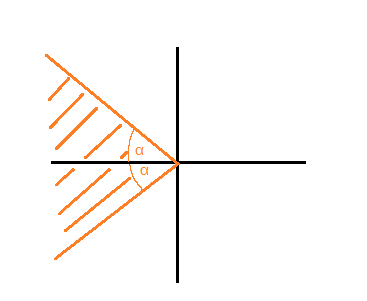
\includegraphics[width=0.3\linewidth]{screenshot021}
				 	\caption{$A(\alpha)$ stability}
				 	\label{fig:screenshot021}
				 \end{figure}
				 
			\end{itemize}
		\end{enumerate}
	\end{definition}
	

\section{Implicit linear multi-step formulas}
These kinds of multi-step methods are conventionally used to numerically solve the systems obtained using modified nodal analysis. Our assumption that we only consider network equations arising from networks consisting of RLC components as well as controlled sources which keep the index between 1 and 2 still holds.

We consider the equations in charge/flux oriented formulation
\begin{align*}
	0 &=
	\underbrace{ 
	\left( \begin{matrix}
		A_c & 0 \\
		0 & I \\
		0 & 0
	\end{matrix} \right)}_{=:A}
	\underbrace{
	\left( \begin{matrix}
		\dot{q} \\
		\dot{\phi} 
	\end{matrix} \right)}_{=:\dot{y}}
	+
	\underbrace{
	\left( \begin{matrix}
		A_R r(A_R^\top u,t) + A_L i_L + A_V i_V + A_I i(u, i_L, i_V, t) \\
		- A_L^\top u \\
		v(u, i_L, i_V, t) - A_V^\top u
	\end{matrix} \right)}_{=:f(x,t)}, \\
	\underbrace{
	\left( \begin{matrix}
		q \\
		\phi 
	\end{matrix} \right)}_{=:y} 
	&=
	\underbrace{
	\left( \begin{matrix}
		q_C(A_C^\top u) \\
		\phi_L(i_L) 
	\end{matrix} \right)}_{=:g(x,t)},
\end{align*}

or simply
\begin{align*}
	0 &= F(\dot{y}(t), x(t), t) :=A \dot{y}(t) + f(x(t),t), \\
	0 &= y(t) - g(x(t)).
\end{align*}
with $x:=(u, i_L, i_V)^\top$ containing the unknowns.

The conventional approach to solve those systems numerically can be split into three main steps:
\begin{enumerate}
	\item Computation of consistent initial values
	
	The first step is to compute consistant inital values $(x_0, y_0)$ at the initial time point $t_0$. In the index-1 case this can be done by solving a so called steady state problem. Steady state means that we consider a not time-dependent circuit (DC operating point). This means we have to solve
	\begin{displaymath}
		F(0,x_0,t_0) = 0
	\end{displaymath}
	
	for $x_0$ and then set $y_0 = g(x_0)$.
	
	\item Numerical integration based on multi-step schemes
	
	Using the consistent initial values we obtain solutions of the network equations at discrete timepoints $t_1, t_2, ...$ by integration with linear multi-step methods.
	
	\item Transformation of the DAE into a nonlinear system of equations. 
	
	The numerical solution is now reduced into solving a system of equations of the form
	\begin{displaymath}
		F(\alpha_k g(x_k) + r_k, x_k, t_k) = 0
	\end{displaymath}
	
	which can be solved iteratively using Newton's method.
\end{enumerate}

In the following two subchapters we will give a short overview over the two most commonly used methods for solving those systems.

\subsection{BDF-schemes}
	chapter 9.2 numerik book
	wikipedia
	
	The most commonly used numerical methods for solving the systems that arise in electrical circuits are the BDF-scheme and the trapezoidal rule. 
	
	We will not give a deeper look into their construction but will only state their properties. BDF schemes are appealing because they save function evaluation as much as possible, since this is very costly in circuit simulation.
	
	The \emph{backward differentiation fooormula (BDF)} is a family of implicit linear multistep methods. They have the general form
	\begin{equation}
		\sum_{k=0}^{s} \alpha_k y_{n+k} = h \beta f(t_{n+s}, y_{n+s})
	\end{equation}

	Since we are interested in the unknown $y_{n+s}$ which is used to evaluate $f$, this method is implicit. The coefficients $\alpha_k$ and $\beta$ are chosen, so that the method achieves order $s$ which is the maximum possible.
	
	The BDF or BDF-k formulas for $k=1,...6$ have the following form
	\begin{align*}
		k = 1 &: h f_{m+1} = u_{m+1} - u_m \\
		k = 2 &: h f_{m+2} = \frac{1}{2} (3 u_{m+2} - 4 iu_{m+1} + u_m) \\
		k = 3 &: h f_{m+3} = \frac{1}{6} (11 u_{m+3} - 18 u_{m+2} + 9 u_{m+1} - 2 u_m) \\
		k = 4 &: h f_{m+4} = \frac{1}{12} (25 u_{m+4} - 48 u_{m+3} + 36 u_{m+2} - 16 u_{m+1} + 3 u_m) \\
		k = 5 &: h f_{m+5} = \frac{1}{260} (137 u_{m+5} - 300 u_{m+4} + 300 u_{m+3} - 200 u_{m+2} +75 u_{m+1} -12 u_m) \\
		k = 6 &: h f_{m+6} = \frac{1}{60} (147 u_{m+6} - 360 u_{m+5} + 450 u_{m+4} - 400 u_{m+3} + 225 u_{m+2} - 72 u_{m+1} + 10 u_m)
	\end{align*}
	
	Methods with $s > 6$ are not zero-stable. Indeed in reality methods with order greater than 3 are rarely used because of their low smoothness properties.
	
	BDF schemes have consistency order $p = k$. They are methods for solving stiff equations, thus their stability is indicated by their region of absolute stability. Unfortunately not all BDF-schemes are A stable, but their stability region still contains a large part of the complex left half-plane (see figure \ref{fig:screenshot020} They are the most efficient linear multistep methods of this kind.
	
	\begin{figure}[H]
		\centering
		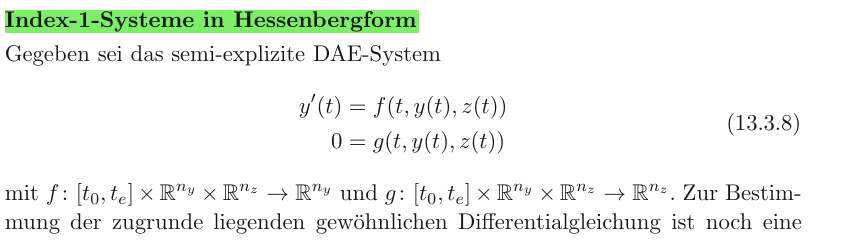
\includegraphics[width=0.7\linewidth]{screenshot020}
		\caption{stability regions of BDF-schemes}
		\label{fig:screenshot020}
	\end{figure}
	
	The first timestep is always performed by BDF1 (implicit Euler scheme) as a starting procedure.
	
	
\subsection{trapezoidal rule}

	The trapezoidal rule is a somewhat natural alternative to BDF2 since it is A-stable and as a linear multistep method of order 2 the one with the smallest leading error coefficient. (\cite{ModellingAndDiscretizationOfCircuitProblems})
	
	It works by approximating the region under the graph of the function $f(x)$ as a trapezoid, hence the name. It follows that	
	\begin{displaymath}
		\int_{a}^{b} f(x) dx \approx (b-a)\frac{1}{2} (f(a)+f(b))
	\end{displaymath}
	
	This procedure is repeated for small subsections of the Intervall $[a,b]$. Thus we obtain the iteration formula
	\begin{displaymath}
		u_h (t+h) = u_h(t) +\frac{h}{2}[f(t,u_h(t)) + f(t+h, u_h(t+h))].
	\end{displaymath}
	
	This iteration rule can also be formulated using the butcher tableau	
	\begin{displaymath}
		\begin{array}{c|cc}
			0 & 0 & 0 \\
			1 & \frac{1}{2} & \frac{1}{2} \\
			\hline
			& \frac{1}{2} & \frac{1}{2}
		\end{array}
	\end{displaymath}
	
	Because $u_h(t+h)$ appears in $f$ again we see that this is an implicit method. The butcher tableau confirms this as well.
	
\section{Numerical Examples}
	
	In this section we will give two explicit examples of circuits being solved using either of the above mentioned methods and compare the convergence speed between the methods as well as comparing the suitability of the methods for systems of different index.
	


		
		
	
	
	